Dado que BFS es una busqueda no informada, se ignoran las heurísticas.\\
Tenemos la siguiente pila:
\begin{center}
    \begin{tabular}{|c|c|c|}
        \hline
        Estado actual & Siguientes estados & Cerrados\\
        \hline
        $s_0$ & $s_2$ & $s_0$ \\
        \hline
        $s_2$ & $s_1, s_4$ & $s_0,s_2$ \\
        \hline
        $s_1$ & $s_4$ & $s_0,s_2,s_1$ \\
        \hline
        $s_4$ & $s_3, s_5$ & $s_0,s_2,s_1,s_4$ \\
        \hline
        $s_3$ & $s_5$ & $s_0,s_2,s_1,s_4,s_3$ \\
        \hline
        $s_5$ & $s_6, [s_7]$ & $s_0,s_2,s_1,s_4,s_3, s_5$ \\
        \hline
        $s_7$ & Estado final encontrado & $s_0,s_2,s_1,s_4,s_3, s_5, s_7$ \\
        \hline
    \end{tabular}
\end{center}
Se tiene el siguiente árbol:
\begin{center}
    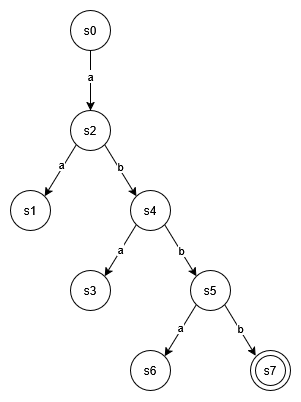
\includegraphics[height = 10cm]{respuestas/img/treeE7b.png}
\end{center}
Por lo que el camino solución es $a,b,b,b$, conformado por los estados $s_0,s_2,s_4,s_5,s_7$.